\section{The \cs\ Algorithm}
\label{sec:architecture}
%\subsection{Data Structures}
The \cs\ algorithm is based on three data structure: (1) the \textit{\sfa}, (2) the \textit{\cs}, and (3) the \textit{\sea}. Figure~\ref{fig:ds} illustrates these data structures.
The algorithm uses the first two to store identifiers of flows suspected as HH flows with different levels of confidence.
In the \sfa\ the algorithm stores identifiers of flows that were recently encountered in order to track their potential growth. When this growth is fulfilled these flows are propagated to the \cs. In the \cs\ the algorithm stores identifiers of ``heavy" flows, i.e., flows that already showed some evidence for a large amount of traffic.

\begin{figure}
  \centering
  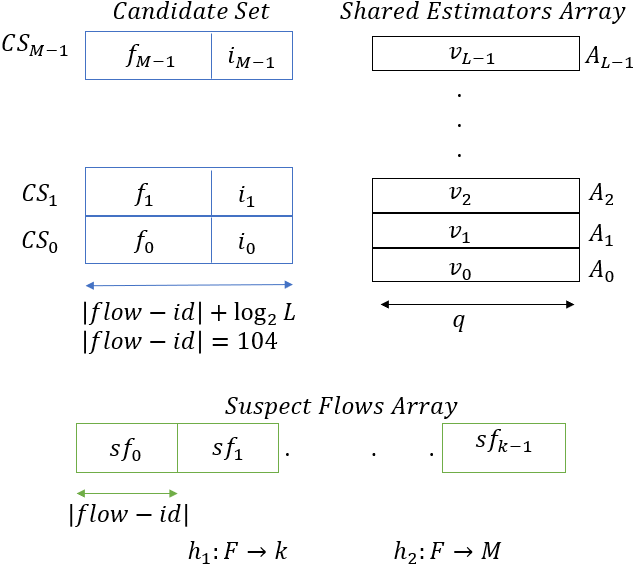
\includegraphics[width=\linewidth]{HH/figures/ds.png}
  \caption{The basic architecture of the \cs\ algorithm}
  \label{fig:ds}
\end{figure}

This way, the algorithm facilities tracking ``recent" and ``heavy" flows to estimate their frequency using the \sea. Next, we describe how a HH flow is handled by the algorithm. First, it is added into the \sfa. Then, on the second arrival of its packets, if it was not evicted in the meantime, it is propagated to the \cs. Afterward, it is tracked in the \cs\ and its frequency is estimated via the \sea.

Non HH flows that are of a negligible size usually reaches only the \sfa\ and are not propagated to the \cs. That is, until a second packet from the flow arrives, many other packets from other flows were already processed and probably have evicted the entry of the original flow from the \sfa. This way, the second arrival of a packet from this flow is considered as a new flow, since the algorithm has no data about this flow, and it will be kept at most in the \sfa\ or even not remembered by the algorithm at all.

Other non HH flows that are not negligible but still are not HH could propagate to the \cs\ from the \sfa. However, it is not enough to propagate to the \cs\ in order to be considered as a HH. A flow size estimation in the \sea\ needs to be above the threshold. The \sea\ mechanism is based on the estimation table introduced in the CEDAR algorithm~\cite{CEDAR} and it guarantees a maximal relative error of $\delta$ for any flow in the \cs, thus our algorithm might produce a false positive only on flows with frequencies in the range$[(1-\delta)\phi N, \phi N]$.

\begin{table}
\caption{A summary of the used notations}
\begin{center}
\begin{tabular}{|c|c|}
\hline
\textbf{Symbol}& \textbf{Meaning}\\
\hline
$m$& total available memory\\
\hline
$m_{CS}$& share of \cs\ memory out of $m$\\
\hline
$m_{SFA}$& share of \sfa\ memory out of $m$\\
\hline
$m_{SEA}$& share of \sea\ memory out of $m$\\
\hline
$\phi$& heavy hitter threshold\\
\hline
$N$& number of packets\\
\hline
$F$& 5-tuple flows Universe\\
\hline
$\delta$& guaranteed relative error\\
\hline
$A_i$& $i^{th}$ shared estimator\\
\hline
$L$& number of shared estimators\\
\hline
$q$& width of an estimator\\
\hline
$v_0$& the minimal estimator\\
\hline
$v$& the "propagation" parameter\\
\hline
$M$& the number of entries in the \cs\\
\hline
$CS_i$& $i^{th}$ flow in the \cs\\
\hline
$k$& the number of entries in the \sfa\\
\hline
$sf_{i}$& the $i^{th}$ entry in the \sfa\\
\hline
\end{tabular}
\label{tab:notations}
\end{center}
\end{table}

%\subsection{Initialization}
The first step of initializing the data structures is to partition the total memory available to the algorithm to the three data structures, $m = m_{CS}+m_{SFA}+m_{SEA}$. The algorithm performance strongly depends on this partition of the memory.

Some partitions are more logical than others. For example, it is intuitive that we are interested in having the \sea\ much smaller than the \cs\ ($m_{SEA} << m_{CS}$). Otherwise, one can hold an exact counter for every flow in the \cs\ without paying the penalty of the relative error introduced by the estimators. The partition between $m_{CS}$ and $m_{SFA}$ is one of the tuning parameters of the algorithm.

\subsubsection{\sea\ Initialization}
In~\cite{CEDAR}, the initialization of the shared estimators' values was based on given $\delta, L$, and starts from $v_0=0$. Then, the rest of the values are calculated in a manner to guarantee the maximal relative error of $\delta$. Since we are interested only in estimating the HH flows, we could start from $v_0=v\phi N$, where $N$ is the number of packets and $\phi$ is the threshold of HH flows, and $v$ is the ``propagation parameter". The motivation behind this initialization is that in the \cs\ we monitor only large flows, thus there is no need to waste space for allocating smaller estimators. The ``propagation parameter" is a key tuning parameter, which affects the initial estimated value of flows that were just propagated to the \cs and controlling its value is important to bound some of the error types as we discuss later.

%\begin{maybeappendix}{\sea}
We show that we can generalize the CEDAR scheme to start from a minimal estimator greater than $0$ without affecting its properties or incurring additional memory and speed costs. For that, we show how to build such a generalized scheme on top of the original scheme with the aid of an additional variable $z$. We denote by $v'_i$ the estimator values of the generalized scheme and by $v_i$ the values of the original scheme.

In order to initialize with $v'_0\neq 0$, we initialize the original scheme and set $z=v'_0$ and $v_0=0$. When querying a flow with estimation of $v_i$, then we return $v'_i=v_i+z$. When probabilistically incrementing a flow's estimator, we do so in the same manner as the original scheme, i,e, by incrementing with probability of $\frac{1}{v_{i+1}-v_{i}}$ which is equal to $\frac{1}{v'_{i+1}-v'_{i}}=\frac{1}{v_{i+1}-z-v_{i}+z}$.

The costs of this modification to the original scheme are: (1) holding the additional variable $z$, (2) a single assignment in the initialization, and (3) a single read of the variable $z$ in each estimation query.

Given $m_{SEA}$ memory for the \sea, we calculate the width of a single estimator to be $q=\lceil \log_{2}(10 \phi N)\rceil$ and $L=\lfloor \frac{m_{SEA}}{q} \rfloor$. This assumes that the maximal value ever achieved by a flow is $10$ times the threshold, while this is usually true and this value is never achieved, we note that the cost of increasing it is logarithmic. Which means that doubling the maximal value increases $q$ by one and reduces the number of estimators, $L$, by a negligible $\lceil\frac{M_{SEA}}{q*(q+1)}\rceil$.

%\end{maybeappendix}

\subsubsection{\sfa\ Initialization}
The \sfa\ is initialized as an empty array without any stored flow id. Furthermore, we initialize a hash function $h_1:F\rightarrow k$, which maps every flow id to its entry in the \sfa.

Given $m_{SFA}$ memory for the \sfa, we calculate the size of the array using $k=\lfloor \frac{m_{SFA}}{|flow\_id|} \rfloor$. Where $|flow\_id|$ is the number of bits needed to store the flow identifier and in the case of IPv4 5-tuple flows of the $<$IP\_SRC, IP\_DST, SRC\_PORT, DST\_PORT, PROTOCOL$>$ its $104$.

\subsubsection{\cs\ Initialization}
The \cs\ is initialized as an empty array that does not hold any flow id and all indexes are initialized to 0. That is, there is no flow that the algorithm thinks is a candidate to be a HH flow and all of the initial estimations are $v_0$. Furthermore, we initialize a hash function $h_2:F\rightarrow M$, which maps every flow id to its entry in the \cs.

Given $m_{CS}$ memory for the \cs, we calculate the size of the set using $M=\lfloor \frac{m_{CS}}{|flow\_id| + \lceil \log_2{L} \rceil} \rfloor$.

%\subsection{Insertion}
The insertion operation is triggered when a packet of a 5-tuple flow is encountered, thus it is important to keep this operation an $O(1)$ internal steps. For a packet from flow $f$, the insertion goes as follows:

with probability $\frac{1}{2v_0}$ perform the following:
  \begin{enumerate}
    \item\label{step:1} if $CS_{h_2(f)} = (f,i)$ for some $i$, perform the following $2v_0$ times:
    \begin{enumerate}
      \item\label{step:1:a} increase $i$ by 1 with probability $\frac{1}{v_{i+1}-v_i}$.
      \item\label{step:1:b} if $i$ reaches $L-1$ perform $ShiftUpEstimators()$ and stop.
    \end{enumerate}
    \item\label{step:2} if not, calculate the index $h_1(f)$:
    \begin{enumerate}
      \item\label{step:2:a} if $sf_{h_1(f)}\neq f$ or $sf_{h_1(f)}$ is $Null$, assign the flow identifier of $f$ to $sf_{h_1(f)}$.
      \item\label{step:2:b} if $sf_{h_1(f)}=f$, then:
      \begin{enumerate}
        \item\label{step:2:b:i} evacuate the entry from the array, $sf_{h_1(f)} = Null$.
        \item\label{step:2:b:ii} if $CS_{h_2(f)}$ is empty then put $(f,0)$.
        \item\label{step:2:b:iii} else perform $EvictFromCandidateSet(f)$.
      \end{enumerate}
    \end{enumerate}
  \end{enumerate}
  
The main idea behind the insertion step is to first check if the current flow is already present in the \cs, if yes then we should increase its estimator. Since we consider one out of $2v_0$ packets, then when increasing the estimation we perform it $2v_0$ times.

If $i$ reaches $L-1$ then this flow was advanced up to the highest estimator in \sea. Thus, there is a need to update the \sea\ to include more estimators and this is performed by $ShiftUpEstimators()$ as follows:
\begin{enumerate}
  \item calculate $v_L$ based on the original CEDAR scheme.
  \item append $v_L$ and pop $v_0$ from the array.
  \item set $v_0$ to the value of the new minimal estimator.
  \item\label{step:4} go over the \cs\ entries and remove flows pointing to the previous minimal value.
\end{enumerate}

In the current architecture step~\ref{step:4} is not an $O(1)$ operation, however, we can simply modify the insertion operation to allow step~\ref{step:4} to be an $O(1)$ operation. Instead of searching for and removing flows from the \cs, we store an additional variable, $y$ that stores how many shifts were already performed. Then when checking if a flow is in the \cs, we also check that its $i$ is bigger than the stored number of shifts. If not, then we consider the entry to be empty and simply overwrite it. This is correct, since if $i<y$ then this flow should have been evicted in the $i^{th}$ $ShiftUpEstimators$ operation.

If the flow we are inserting in is not in the \cs\ then we check if it is in the \sfa. If the flow is not in the \sfa\ then we add it the appropriate entry, $sf_{h_1(f)}$. This way we store for future appearances of packets from this flow, that this flow is ``recent" enough. We note that adding a flow to the \sfa\ might evict other flows that share the same hash entry.

If it is already in the \sfa\ then we propagate it to the \cs\ if its entry in the \cs\ is indeed empty. When propagating we set the initial estimation to be $v_0 \neq 0$, the reason for this estimation is that we insert it after two packets, that did not have a hash collision in between their appearances, and all packets are sampled with a probability of $\frac{1}{2v_0}$.

However, it is possible that such propagated flow will be hashed to an already allocated entry, in this case we should decide if to evict the older flow. The algorithm decides on the eviction with probability of $\frac{v_0}{v_i}$ where $v_i$ is the estimation of the older flow. This is described in $EvictFromCandidateSet(f)$ as follows:
\begin{enumerate}
  \item get $(g,i)=CS_{h_2(f)}$
  \item with probability $\frac{v_0}{v_i}$, set $CS_{h_2(f)}=(f,i)$
\end{enumerate}

The motivation behind this probabilistic eviction is that the potential to-be evicted flow had already gained some significant amount of packets previously, and simply evicting it might be the wrong decision. Thus, we evict it only if the new flow has a comparable amount of packets. That is, in expectation it requires $v_i = \frac{1}{ 2\frac{1}{2v_0}\frac{v_0}{v_i}}$ packets to replace the old flow, and that is why we insert the new flow with the same current estimation of the old flow and not with the minimal estimation.


%\begin{maybeappendix}{query}

\subsection{Query a specific flow}
When querying a specific flow, the algorithm calculates $h_2(f)$ and checks if $CS_{h_2(f)}=(f,i)$ for some $i$, if yes it returns $v_i$.

For flows that are not present in the \cs\ the algorithm returns  since it provides no guarantee on the relative error of non HH flows.

\subsection{Query all Heavy Hitter Flows}
When querying the data structure for the HH flows, the algorithm searches the \sea\ for the index of the minimal estimator of value higher than $(1-\delta) \phi N$. Then, it extracts all tuples $(f, i)$ with $i's$ higher than that index. Each tuple means that the flow $f$ has an estimation of $v_i$.

We note that the step of finding the index of the minimal estimator with a value higher than $(1-\delta) \phi N$ is not an $O(1)$ operation. However, since this query usually happens offline, it is not a major issue. To support an $O(1)$ version of this query, it is possible to have an extra variable holding the current index of the minimal estimator with a value higher than $(1-\delta) \phi N$ at the initialization of the \sea\ and update it in every $ShiftUpEstimators()$ operation.

%\end{maybeappendix}